\documentclass[twocolumn]{IEEEtran}
\renewcommand\IEEEkeywordsname{Palabras Claves}
\usepackage{cite}
\usepackage[utf8]{inputenc}
\usepackage{graphicx}
\usepackage{graphics}
\usepackage[spanish]{babel}
\usepackage[cmex10]{amsmath}
\interdisplaylinepenalty=2500
\usepackage{pgfplots}
%\usepackage{algorithmic}
\usepackage{array}
\usepackage{mdwmath}
\usepackage{mdwtab}
%\usepackage{eqparbox}
\usepackage[tight,footnotesize]{subfigure}

\begin{document}
%% Se puede usar \\ para darle el formato deseado
\title{Midgard}
%%%%%%%%%%%%%%%%%%%%%%%%%%%%%%%%%%%%%%%%%%%%%%%%%%%%%%%%%%%%%%%%%%%%%%%%%%%%%%%%%%%%%%%%%%%%%%%%%%%%%%%%%%%%%%%%%%%
% una imagen

%\begin{figure}[h!]
%\centering
%\includegraphics[width=\columnwidth]{NOMBRE.png}
%\caption{DESCRIPtION}
% \label{fig:crossover}
%\end{figure}
%\ref{fig:crossover}   
%THIS is for making a citation of the image otuside the declaration


%hacer una tabla:

%\begin{table}[h!]
%\centering
%\caption{Teorema de Thévenin y Norton}
%\begin{tabular}{c c c c c}
%\hline
%{\bf Rcar(Kohm)}&{\bf Corri.teór$[mA]$}&{\bf Corri.exp$[mA]$}&{\bf Pot.teó$[mW]$} &{\bf Pot.exp$[mW]$} \\ \hline
%{$0,4579$}&{$2,50$}&{$2,20$}&{$2,86$}&{$2,22$}\\
%{$0,9140$}&{$2,09$}&{$2,03$}&{$3,99$}&{$3,77$}\\
%{$1,376$}&{$1,80$}&{$1,82$}&{$4,46$}&{$4,56$}\\
%{$1,837$}&{$1,56$}&{$1,42$}&{$4,47$}&{$3,70$}\\
%{$2,280$}&{$1,39$}&{$1,45$}&{$4,40$}&{$4,80$}\\
%{$2,746$}&{$1,25$}&{$1,21$}&{$4,29$}&{$4,02$}
%\end{tabular}
%\end{table}


%hacer una grafica:

%\begin{tikzpicture}
%\begin{axis}[
%    title={Gráfico P Teórica vs R$_L$},
%    ylabel={Potencia [mW]},
%    xlabel={Resistencis [ohmios]},
%    xmin=0, xmax=3,
%    ymin=0, ymax=5.1,
%    xtick={0, 0.5, 1, 1.5, 2, 3},
%    ytick={0, 1, 2, 3, 4, 5},
%    legend pos=north west,
%    ymajorgrids=true,
%    grid style=dashed,
%]
 
%\addplot[
%    color=blue,
%    mark=square,
%    ]
%    coordinates {
%    (0.4579, 2.86)(0.9140, 3.99)(1.376, 4.46)(1.837, 4.47)(2.280, 4.40)(2.746,4.29)};
%\end{axis}
%\end{tikzpicture}


%% Los autores y su respectiva afiliacion, se usa ~ para evitar que corte la linea
\author{Abraham Arias\\
        e-mail:ipseabraham@gmail.com\\
        Fabian Solano\\
        e-mail:fasm2296@gmail.com
        Lenin Torres\\
        e-mail:ttvleninj@gmail.com\\
        Mauricio Montero Jiménez\\
        e-mail:maumonteroj@gmail.com\\
}

\makeatletter
\def\markboth#1#2{\def\leftmark{\@IEEEcompsoconly{\sffamily}\MakeUppercase{\protect#1}}%
\def\rightmark{\@IEEEcompsoconly{\sffamily}\MakeUppercase{\protect#2}}}
\makeatother
%% Encabezado del Articulo
\markboth{Abraham Arias, Fabian Solano,Lenin Torres, Mauricio Montero}{}
\maketitle

%% menor de 3 parrafos, contiene teoria, actividades y conclusion.
\section{Abstract}

Machines can't improvise well, because you can't program a fear of death (Interstellar 2014), our work is to challenge this affirmation, by the use of genetic algorithms in c++, which is the nearest approach of all the members of the group have been to any kind of artificial intelligence.\\ 
This document covers from the basic steps in the creation of a genetic algorithm, to any analysis to accomplish improvements by intense testing of our software. In addition we also explain how we handle hardware to create random numbers.\\
This genetic algorithm will represent villages including as many logical details according to reality (mutation, randomness, among others) and fantasy as possible. This towns are formed by many individuals with particular behaviors such as monogamy, life time, superstition, reproduction and many more, to ensure that their genetic information survives.



\section{Introduction}
WRITE THIS SECTION AT THE END!\\ \\
Our code will represent concurrently each time a given number of different civilizations, they have a unique goal reproduce as many times as possible, combining genetic information, until the reach at top line, later we will explain the reason of existence of this peak. Until a given time comes, the natural selection process will be tested, all the villages fight against the gods, and that defines if we get a solution by our genetic code.


\section{User Manual}



\section{Libraries and functions}

	\begin{enumerate}
    
    	\item Standard Library in C ++ \\
        C is a general-purpose, procedural, imperative computer programming 
        language developed in 1972 by Dennis M. Ritchie at the Bell Telephone 
        Laboratories to develop the Unix operating system. The C Standard 
        Library is a set of C built-in functions, constants and header files  
        like <stdio.h>, <stdlib.h<math.h>,etc. This library will work as a
        reference manual for C programmers.\\
    
        \item stdint.h\\
        This header was introduced in C99. to allow programmers to create integer 
        types more portable. This types have previously defined their sizes.\\ It is 
        possible to classify them into two kinds, the signed and unsigned, this 
        classification is visible from their type name. The range of widths are from 
        eight bits to the maximum size of a integer.\\
    
        \item Libserial\\
        It provides a collection of C++ classes that allow one to serial ports on 
        POSIX systems like standard C++ iostream objects. With this library we 
        successfully achieve:
        \begin{enumerate}
        \item Simplified serial port programming in C++ under POSIX operating systems\
        \item Support for USB-serial converters.\
        \item Access serial ports from scripting languages such as 									
        PHP, Python, Perl, Ruby, and Java (coming soon in version 0.6.0).\
		\end{enumerate}
            
         \item Tinyxml 1 \\
         Is a simple, small, C++ XML parser that can be easily integrating into other programs. In 
         brief, TinyXML parses an XML document, and builds from that a Document Object Model (DOM) that 
         can be read, modified, and saved.\\
         
         \item POSIX library.S unistd.h - standard symbolic constants and types.\\
         The <unistd.h> header defines miscellaneous symbolic constants and types, and declares 
         miscellaneous functions.\\
            
         \item Rand \\
         Returns a pseudo-random integral number in the range between 0 and max value. This number is 
         generated by an algorithm that returns a sequence of apparently non-related numbers each time 
         it is called. This algorithm uses a seed to generate the series, which should be initialized 
         to some distinctive value using function srand.\\
            
         \item fstream \\
         Input/output stream class to operate on files. Objects of this class maintain a filebuf object 
         as their internal stream buffer, which performs input/output operations on the file they are 
         associated with (if any). File streams are associated with files either on construction, or by 
         calling member open.\\
         
         \item OpenCv
         OpenCV is released under a BSD license and hence it’s free for both academic and commercial 
         use. It has C++, C, Python and Java interfaces and supports Windows, Linux, Mac OS, iOS and 
         Android. OpenCV was designed for computational efficiency and with a strong focus on real-time 
         applications. Written in optimized C/C++, the library can take advantage of multi-core 
         processing. Enabled with OpenCL, it can take advantage of the hardware acceleration of the 
         underlying heterogeneous compute platform. Adopted all around the world, OpenCV has more than 
         47 thousand people of user community and estimated number of downloads exceeding 9 million. 
         Usage ranges from interactive art, to mines inspection, stitching maps on the web or through 
         advanced robotics.

	\end{enumerate}



\section{Data structures}

	\begin{enumerate}
		\item Generic Circular Linked List\\
        
        Is the same definition of a linked list, but now it is double connected and also the 
        tail contains a pointer to the head, this is his particular characteristic.
     	   \begin{figure}[h!]
				\centering
				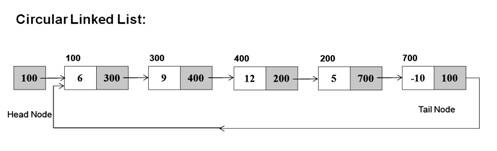
\includegraphics[width=\columnwidth]{src/circularLinkedList.jpg}
				\caption{Circular Linked List}
			\end{figure}\\
		Other particular characteristic is that this data structure it is able to handle any 
        kind of objects inside, thanks to the use of templates.
        
	\end{enumerate}
    
    
    
    
\section{Algorithms}
Our genetic algorithm as any other follow a series of steps like any other, first we create the initial
population, and insert them into a loop, where we calculate the fitness first, then select the fittest to reproduce, and finally select which ones stay and which others continuous alive.\\* 
    \begin{figure}[h!]
	\centering
	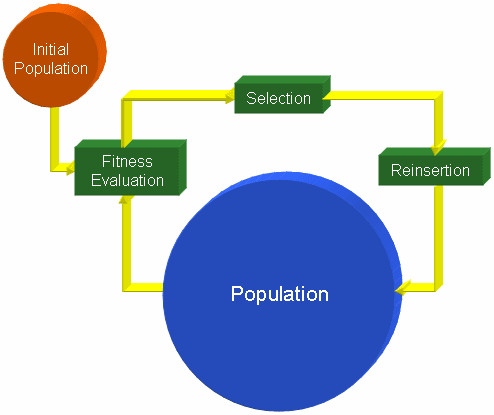
\includegraphics[width=\columnwidth]{src/GAalg.jpg}
	\caption{Steps of GA}
	\end{figure}
    
\begin{enumerate} 
	\item Fitness
    After just created the first generation, proceed with the function fitness, which is different 
    according to the individual's population, due to need to increase specific attributes in each 	
    population. But the main idea consist in divide one by one attribute of the individual between the 
    sum of all those attributes in the whole population, finally do this for the 8 characteristics and 
    put it together in number called fitness. 
        \begin{figure}[h!]
        \centering
        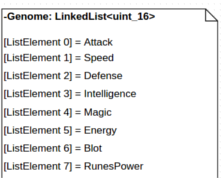
\includegraphics[width=\columnwidth]{src/cualidades.png}
		\caption{Steps of GA}
		\end{figure}\\
    As each population have more value attributes, we need to calculate separately fitness for each  
    population, a more detail explanation is available in section ~\nameref{sec:Implemented methods}.
        
        
    \item Crossover
    	Inspired in nature, we combine two possible solution, one from the mother and other from the 
        father to create a new offspring with similar attributes.
	    \begin{figure}[h!]
        \centering
        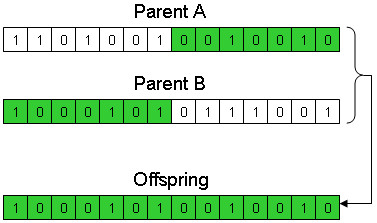
\includegraphics[width=\columnwidth]{src/crossover.jpg}
		\caption{Steps of GA}
        \label{fig:crossover}
		\end{figure}
        We work with a simple crossover as the figure \ref{fig:crossover} shows, in which we take half 
        chromosome from the mother and the father and by a simple operations with masks and with 
        logical operators achieved the half and half combination. It is known that specific crossover
        help in particular cases, however in this project by the moment we keep this operation simple
        unless future testing proves deficiencies or needs of change in this area. 
        
        
    \item Mutation and Inversion
    \item  Random numbers
    
\end{enumerate}


\section{Implemented methods} \label{sec:Implemented_methods}
	\begin{enumerate}

	\item Fitness 
    
\end{enumerate}
    



\section{Techniques of algorithm's designs}




\section{Results}

\begin{enumerate}
	\item Circuit of random numbers generator. 

\end{enumerate}






\section{Design patterns}

\section{Known Issues}

\section{Activities by student}

\section{Encountered problems}
\begin{enumerate}
	\item Lib serial installation\\
    The first attempt to install it through the two first links, was not enough. At this 
    point we realize it is necessary to declare the next line at the very beginning of 
    the main:
    \begin{center}
 	   \begin{verbatim}
			    using namespace LibSerial;
		\end{verbatim}

	\end{center}
 	After doing this, the compiler we us an \textit{-lserial} alert. The solutions 
    appears to be, introduce the same word as a flaf in the compiler. Then an \textit{ 
    Undefined reference to (any method of lib serial)}, so we add the word 
    \textit{serial} to the GCC C++ linker, what did solve our problem. This library was 
    required to read data from an Arduino, which at the same time reads information from 
    our circuit generator of random number.\\

	\begin{center}
    Bibliography
    \end{center}
	How to install libserial-dev package in Ubuntu Utopic. (n.d.). Retrieved May 3, 
    2015, from http://www.howtoinstall.co/en/ubuntu/utopic/universe/libserial-dev/ \\*
    Libserial Package, debain. (n.d.). Retrieved May 3, 2015, from
    http://superuser.com/questions/110317/libserial-package-debain  \\*
    Thread: Undefined reference when linking SerialStream. (n.d.). Retrieved May 3, 
    2015, from http://forums.codeguru.com/showthread.php?459303-undefined-reference-when-
    linking-SerialStream \\*
    User3536692: LibSerial Eclipse Ubuntu. (n.d.). Retrieved May 3, 2015, from 
    http://kalkanotel.com/libserial-eclipse-ubuntu-i466915.htm \\*
    Errors using LibSerial. (n.d.). Retrieved May 3, 2015, from 
    http://stackoverflow.com/questions/25286648/errors-using-libserial \\*
    Interfacing Arduino with C and libSerial. (2008, August 4). Retrieved May 3, 
    2015, from http://sglez.org/2008/08/05/interfacing-arduino-with-c-and-libserial/ \\*
    
    
	\item The main crashed\\
    In a given moment our main stopped working, we were suggested not to initialize cons 
    to null, but in no place we were doing it, however we actually were setting a static 
    variable to 0, just we avoided doing that, everything keep working.
    \begin{center}
    Biblliography
    \end{center}
    How to avoid the error: Terminate called after throwing an instance of 
    'std::logic error' what(): Basic string:: S construct null not valid. (n.d.). 
    Retrieved May 3, 2015, from http://stackoverflow.com/questions/11705886/how-to-avoid-
    the-error-terminate-called-after-throwing-an-instance-of-stdlog\\*


	\item How to handle decimals form in the fitness function\\
    	At the moment to calculate the fitness for each individual, the division 
        operation is required, And always we have a smaller numerator than the 
        denominator, this causes numbers smaller than 1, an integer can not handle this 
        propertly, so the solution taken, uses the float data type.
    \begin{center}
    Biblliography
    \end{center}
    Std::setprecision. (n.d.). Retrieved May 3, 2015, from 
    http://www.cplusplus.com/reference/iomanip/setprecision/\\*
	
    \item Too many initializers c++ array \\
    	To send a 1 to the arduino we have to options. It is possible to make the arduino 
        to read until no more information is send. And the second one, the one we choose, 
        is to interpret the data we want to send a is in the ascii code. For example to 
        send the number 10, we just send the : character, and so on.\\*
        To assing each number to their respective character, anarray of 16 positon was
        created. But in compiling time we get the error: \textit{too many initializers 
        to array}. We choose to ignore that 
        
    \begin{center}
    Biblliography
    \end{center}
    Too many initializers for 'int [0]' c. (n.d.). Retrieved May 3, 2015, from 
    http://stackoverflow.com/questions/21152171/too-many-initializers-for-int-0-c\\*

	\item The Arduino is too slow\\
    At the beginning we sent a single number, that indicates the number if bits to form a number, in 
    this attempt we force the arduino to do all the shifts and comparisons, but take too much time 
    
    \item El generador de números aleatorios no genera el último número para 3 bits, 
    para números mayores a 3 bits no se genera los números mayores a x=2n-n\\
	
\end{enumerate}

\section{Conclusions}
\begin{enumerate}
    \item C1
    \item C2
\end{enumerate}



\section{Bibliography}

\section{Class diagram and SVN}

	The class diagram is attached with this document.\\
    
    All our code is free and available at:\\ https://github.com/Abrahamon/M1dg4rt.git \\ 



\bibliographystyle{IEEEtran} %%Carga el estilo para la Bibliografia
\bibliography{mybibfile}    %%% Crea la Bibliografia a Partir de la Base de Datos mybibfile.bib

\end{document}
